\chapter{Authenticity Proofs}\label{chap:chap3}

\section*{}

In this chapter, the author takes a deep dive into existing authenticity mechanisms, in terms of their applicability and limitations.

In the context of today's Web, we are accustomed to trusting that a certain website or data is originated from the expected source due to the general adoption of the HTTPS protocol. An extension of the HTTP protocol which creates an encrypted and authenticated channel between the client and the web-server providing the requested information. Then it becomes a matter of whether we trust the source or not, but no doubts are raised as for the channel through which we received it.

Unfortunately, in the context of blockchain, the most used, available and trusted protocols do not have a direct way of communicating with HTTPS enabled services and therefore obtain authenticated data. This creates the need for a trusted service to input that information, but trusting in a third-party service requires it to provide irrefutable proof of its honesty.

Oracles, currently resort to two main techniques to prove their honesty. (1) Authenticity proofs, which is a software or hardware generated cryptographic proof during or after an execution that can later be used to prove the integrity and honesty of the execution or of the provided data. (2) Trusted Execution Environments (TEE) which add another layer of security by isolating the application code from the environment in which it ran, and may also provide cryptographic proof of their honest behaviour.

\section{Trusted Execution Environment (TEE)}
A Trusted Execution Environment is a secure computational environment that is strongly isolated from the main operating system. It provides application isolation, integrity and memory confidentiality. Sensitive data is stored, processed and protected from the main operating system or network. This isolation is accomplished through software and hardware-enforced mechanism. TEE runs a small operating system which exposes a minimal interface to the running application and therefore reduces the attack surface. Advanced TEE embeds unique identities that allow to verify the device authenticity and can be used to generate proofs of the device honest execution.

Examples of TEEs are Intel Software Guard Extensions (SGX)~\footnote{More information on Intel SGX can be found here: https://software.intel.com/en-us/sgx/sdk} and ARM Trustzone-based Secure Elements~\footnote{ARM whitepaper on ARM Trustzone-based TEE can be found here: https://www.arm.com/files/pdf/TrustZone-and-FIDO-white-paper.pdf}, the latter is commonly found on smartphones. Another example is Trusty~\footnote{More information on Trusty can be found here: https://source.android.com/security/trusty}, a secure Operating System (OS) that provides a TEE for Android. It is isolated from the rest of the system by both hardware and software. Trusty's isolation protects it from malicious apps installed by the user and potential vulnerabilities that may be discovered in Android.

% FXIME: Confirmar se estas referencias em footnote deveriam estar em referencia mesmo no final

\section{Authenticity Proofs Mechanisms}

Several authenticity mechanisms have been developed and, as described in the state-of-the-art revision, most oracles as a service providers use authenticity proofs to prove their honest behaviour. However, these proofs are not infallible and the details or their implementation are not always transparent or do not provide the disclosed level of trust. I will deep dive on the most common proofs and discuss their implementation and applicability.

\subsection{TLSNotary}\label{proof:TLSNotary}

% FIXME: devias explicar sucintamente como funciona o HTTPS e o que é o TLS. o sítio certo para isso talvez seja a secção seguinte, e talvez nem seja preciso mesmo mencionar TLS aqui.  Ambos estes acronimos (HTTPS e TLS) deviam aparecer por extenso nalgum ponto. quando explicares em que consiste o TLS, explca também o papel desta master key

TLSNotary is a mechanism for independently audited HTTPS (Hyper Text Transfer Protocol Secure) sessions. Allowing clients to provide evidence to a third party auditor that certain web traffic occurred between himself and the server. This mechanism takes leverage of the TLS (Transport Layer Security)~\footnote{Information on the TLS protocol can be found here: https://www.ietf.org/rfc/rfc2246.txt} handshake protocol to create an irrefutable proof, as long as the auditor trusts the server's public key, by splitting the TLS master secret~\footnote{The master secret is used, when generating keys and MAC secrets, as an entropy source, and the random values provide unencrypted salt material and IVs for exportable ciphers.} between three parties: the server, the auditee and the auditor.

The algorithm allows an auditor to verify some part of a session by withholding a small part of the secret data used to set up the HTTPS connection while allowing the client to conduct an HTTPS session normally. The auditor never fully possesses, at any time, any of the session keys and therefore cannot decrypt any sensitive information and can only verify that certain traffic did occur.

\subsubsection{How it works}
TLSNotary modifies the TLS handshake protocol on the client side by levering some properties of TLS 1.0 and 1.1. More specifically the pseudorandom function (PRF) used in the TLS 1.0 RFC 2246.

\begin{ceqn}
    \begin{align}
        PRF(secret,label,seed) = P_MD5(S1,label+seed) \otimes P_SHA-1(S2,label+seed)
    \end{align}
\end{ceqn}

This function compromises two secrets, S1 and S2. The auditor and auditee will independently generate random bytes of data, S1 and S2, respectively.

The auditee applies P\_MD5 to S1, generating 48 bytes:

\begin{ceqn}
    \begin{align}
        H_{1} = H_{1,1} \parallel H_{1,2}
    \end{align}
\end{ceqn}

The auditor applies P\_SHA-1 to S2, generating 48 bytes:

\begin{ceqn}
    \begin{align}
        H_{2} = H_{2,1} \parallel H_{2,2}
    \end{align}
\end{ceqn}


The auditor and auditee then exchange H21 and H12 allowing each other to construct different halves of the master secret, M2 and M1, respectively.

\begin{ceqn}
    \begin{align}
        M_{2} = H_{1,2} \parallel H_{2,2}
    \end{align}
\end{ceqn}

\begin{ceqn}
    \begin{align}
        M_{1} = H_{2,1} \parallel H_{1,1}
    \end{align}
\end{ceqn}

The auditee and auditor calculate X and Y, respectively.

\begin{ceqn}
    \begin{align}
        X = P\_MD5(M_{1})
    \end{align}
\end{ceqn}

\begin{ceqn}
    \begin{align}
        Y = P\_SHA-1(M_{2})
    \end{align}
\end{ceqn}

The auditor sends sufficient bytes from Y to the auditee so that it can compute the necessary encryption keys and client mac key to send the request to the server.

Then the server response is received, but not decrypted, and the network traffic is logged and a hash of the traffic is computed and set to the auditor as commitment.

Only then, does the auditor send the remaining bytes of Y to the auditee and this allows him to calculate the server mac key and safely execute the regular TLS decryption and authentication steps.

This complex sequence of calculations prevents the auditee from creating a fake version of the post-handshake traffic from the server since he did not have in his possession the server-mac-write-secret to decrypt and authenticate the initially requested data.

A more detailed flow and explanation can be consulted in the TLSNotary white-paper \cite{TLSNotary}.



\subsubsection{Limitations}
TLSNotary provides some capabilities to attest TLS connections but comes with several limitations. Firstly, TLSNotary supports only TLS 1.0 or 1.1, the properties mentioned before are not present in TLS 1.2 and 1.3 and the former are considered less secure versions of TLS. Secondly, TLSNotary depends on RSA Key exchange, which does not provide forward secrecy. Thirdly, TLSNotary uses MD5 and SHA-1 functions, which are now considered deprecated. Finally and most importantly, TLSNotary requires trusting in a third party in most of its implementations, such as in Oraclize~\cite{Oraclize}, and being an interactive proof there is no way to verify the TLSNotary proof unless you were performing the role of the auditor during the retrieval. Oraclize, runs an auditor node on Amazon Web Services (AWS), claiming that this implementation is secure as far as AWS is trusted, simply moving the trust to a larger central entity. It also only allows the existence of one auditor in which we must trust, TLSNotary will not be a suitable solution if more than one auditor is required.


\subsubsection{Conclusions}
The TLSNotary proof is promising due to be software based and is, as of this moment, the most spoken of authenticity proof. However, it's applicability is increasingly getting limited due to the deployment of new TLS versions and the assurances provided by the proof current implementations, which simply move the trust to a bigger entity. Therefore, it should not be considered a reliable authentication method for future implementations.

\subsection{Android Proof}
%FIXME: add references

In the oracle context, the Android Proof \footnote{Documented explanation of the proof can be found here: https://provable.xyz/papers/android\_proof-rev2.pdf} results from Oraclize research and development efforts. It takes leverage of SafetyNet software attestation and Android Hardware Attestation to provision a secure and auditable environment to fetch authenticated data.

\subsubsection{SafetyNet Attestation}
SafetyNet~\footnote{Further described on the google developer page: https://developer.android.com/training/safetynet/attestation.html}, developed by Google, is an API service that allows assessing the Android device in which an app is running on. It provides a cryptographically-signed attestation, assessing the integrity of the device, looking at the software and hardware environment for integrity issues. By returning an SHA-256 hash of the application that called the SafetyNet API it allows assessing if the application running on the device has not been tampered with by comparing the application SHA-256 hash with its publicly available and distributed open-source code.

\subsubsection{Android Hardware Attestation}
Since Android Nougat~\footnote{https://www.android.com/versions/nougat-7-0/}, developers are able to generate an hardware attestation object with details regarding the device unique key stored in the Android Hardware KeyStore~\footnote{Further explanation can be found here: https://source.android.com/security/keystore/}. The attestation object is signed by a special attestation key kept on the device and the root certificate used by that key is a known Google certificate. This guarantees that the hardware running the code has not been tampered with.

\subsubsection{How it works}
The application running on the Android device, on its first run, creates a NIST-256p key pair, containing the Hardware Attestation Object to prove the integrity of the key, using the Android Hardware KeyStore.

When a request is sent to the Android device, it starts an HTTPS connection and the entire HTTP response is retrieved. The response's SHA256 hash is signed using the hardware attested key pair created on the application start. A call to SafetyNet API is then issued to attest the SHA-256 hash of the application package running on the device, which should be open-source and public available and distributed, guaranteeing the application integrity and therefore that no change has occurred on the HTTP response before it was signed and its hash used in the SafetyNet request.

SafetyNet then returns an attestation response in the JSON Web Signature format (JWS) that guarantees the integrity of the application running, the integrity of the system in which the application ran and that both the HTTPS request and the signing process using the initially created and attested key has taken place in the application issuing the SafetyNet request.

The SafetyNet JWS response and the HTTP response is sent back for off-chain verification and validation.

\subsubsection{Conclusions}
The Android proof is a far more complex and in-depth authenticity proof in comparison to TLSNotary. It provides strong guarantees of software and hardware integrity as well as of the requested data. Nonetheless, it relies on a centralized authority, Google, to develop a secure Trusted Execution Environment (TEE), used by Android to generate private keys, and to maintain SafetyNet security sophisticated enough to offer good guarantees of the device and application integrity. A bottleneck in this approach can be the required use of a physical Android device, limiting the scalability context of this approach, but nonetheless, as long as Google is trustworthy it is a very secure model.

\subsection{Ledger Proof}

The ledger proof is based on the use of a specific trusted environment, the Ledger Nano S~\footnote{https://shop.ledger.com/products/ledger-nano-s} and Ledger Blue~\footnote{https://shop.ledger.com/products/ledger-blue}, developed by a French company to secure crypto assets safely. This device provides an attestation for its authenticity and code integrity.

\subsubsection{How it works}

This device implements several layers of hardware and software to prove the security of its execution. These devices run specific software, BOLOS~\footnote{Specific information regarding BOLOS can be found here: https://ledger.readthedocs.io/en/0/bolos/index.html} (Blockchain Open Ledger Operating System), which has an SDK that enables developers to build application which can be installed on the hardware. BOLOS exposes a set of kernel-level APIs which allows running secure cryptographic operations as well as attest the device and the code running on it. The later is very useful as it allows to run code in a secure manner and provides an attestation for the code. An application can ask the kernel to produce a signed hash of the application binary code. A special attesting key is used in this process and is safely controlled by the kernel, away from attacks attempts by any application code. With this, the ledger proof leverages both the device attesting and code attesting features to prove that the applications are running on a TEE of a ledger device.

\subsubsection{Conclusions}

Currently, the ledger proof is used by Oraclize to provide true random data to a smart contract. But its use can be extended to other computation operations that may require to run outside of the blockchain as long as there is support in terms of computational and memory capacity by the ledger device. The device also lacks a direct connection to the internet and therefore cannot be used to query data from the internet.


\subsection{TLS-N}

TLS-N \cite{Ritzdorf2017}, is the first privacy preserving TLS extension that is efficient and most importantly provides non-repudiation~\footnote{Non-repudiation refers to a state of affairs in which the authenticity of something cannot be challenged, meaning that there is absolute guarantee that something happened the way that it is stated.}. TLS-N does not require the use of a third-party or any trusted hardware and is an extension to the TLS 1.3 protocol. In comparison to other implementations such as TLSNotary which rely on deprecated versions, is up to date to the current technologies.
It guarantees non-repudiation, not only in a single TLS message exchange but also in a conversation compromising several messages. It allows, with an additional computation overhead, to obfuscate certain parts of the conversation (such as passwords or other sensitive information) while keeping its trust model intact.

In the TLS-N model, there is no need to trust in a single auditor, such as in TLSNotary, since the proofs are non-interactive and can be inspected by anyone, at any point in time, without having to trust in a single auditor honesty.


\subsubsection{How it works}
TLs-N requires the web server (generator) and the client (requester) to have both support for the protocol.

Initially, both generator and requester establish a TLS connection and negotiate the TLS-N parameters in the handshake. The generator stores the state of the conversation which comprises a hash value incorporating all previous records, an ordering vector and the time stamp from the start of the session.

The protocol ends when the requester sends a request for evidence. The evidence is composed of a window of the exchanged ordered messages signed by the generator. The window begins right after the handshake, this prevents Content Omission Attacks, depicted on Figure~\ref{fig:/figures/tlsn-content-omission}.

\begin{figure*}[h]
    \begin{center}
      \leavevmode
      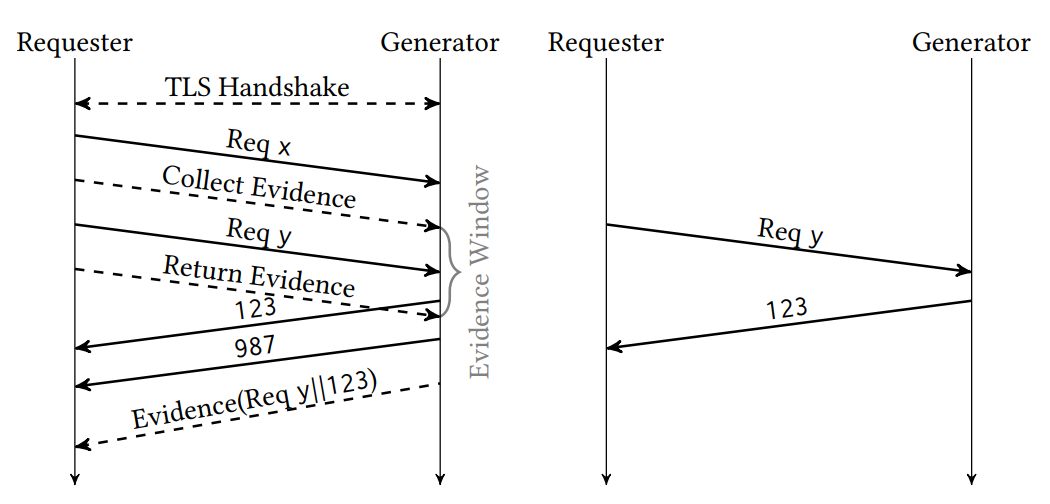
\includegraphics[width=0.9\textwidth]{figures/tlsn-content-omission.PNG}
      \caption{Content Omission Attack - The left figure shows the original and the right figure the signed conversation.}{Image extracted from \citet{Ritzdorf2017a}}
      \label{fig:/figures/tlsn-content-omission}
    \end{center}
\end{figure*}

In this situation the evidence collection only starts after the first request is done, and another request is asked right after (this one, inside the window collection, Req y on the image) and the response for the first request is assumed to be the response to the second one. Only this two messages are stored in the evidence window, since context is missing in the signed conversation, the response 123 appears to belong to request y which is incorrect. Therefore, TLS-N always starts right after the TLS handshake. The correct TLS-N flow is presented on Figure~\ref{fig:/figures/tlsn-normal-flow}.


\begin{figure*}[h]
    \begin{center}
      \leavevmode
      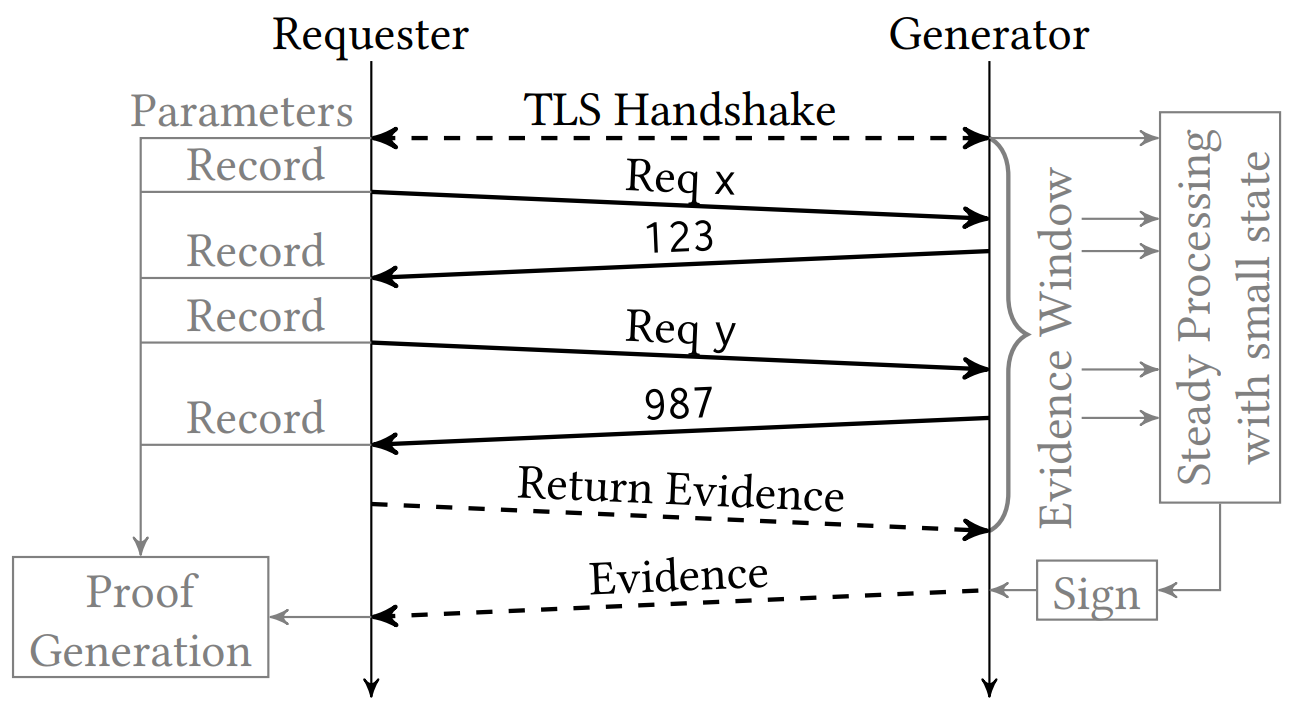
\includegraphics[width=0.7\textwidth]{figures/tlsn-normal-flow.PNG}
      \caption{Simplied Overview of TLS-N.}{Image extracted from \citet{Ritzdorf2017a}}
      \label{fig:/figures/tlsn-normal-flow}
    \end{center}
\end{figure*}

To generate a small proof independently of the number of messages, TLS-N uses merkle trees~\cite{MerkleTrees} to create a chain of messages' hashes and then returns only the last hash, which to be created requires all the previous hashes. This ensures a small storage overhead per TLS session.


\subsubsection{Conclusions}
TLS-N was designed with the oracle trust problem in mind, the generated proof is small enough to be evaluated on-chain on a smart-contract. The only drawback is that the smart contracts cannot verify TLS signatures based on the web-PKI (public-key infrastructure) and therefore the contract must have the generator public key.

TLS-N is, therefore, a promising solution to the oracle trust problem being the only major drawback requiring the data providers to adopt the TLS-N protocol.


\subsection{Town Crier}

Town Crier~\citet{Zhang2016a} (TC) authenticates data-feeds through the use of trusted hardware, more specifically Intel SGX enabled CPUs. By levearing intel SGX, and as long as this system is trusted, there's is no need to trust the environment in which TC is running since it the TEE guarantees the isolation of the TC implementation.

Thanks to its use of SGX and various innovations in its end-to-end design, Town Crier offers several properties that other oracles cannot achieve:

\begin{enumerate}
    \item \textbf{Authenticity guarantee}: There's no need to trust any particular service provider(s) in order to trust Town Crier data. (You need only believe that SGX is properly implemented.)
    \item \textbf{Succinct replies}: Town Crier can prune target website replies in a trustworthy way to provide short responses to queries. It does not need to relay verbose website responses. Such succinctness is important in Ethereum, for instance, where message length determines transaction costs.
    \item \textbf{Confidential queries}: Town Crier can handle secret query data in a trustworthy way. This feature makes TC far more powerful and flexible than conventional oracles.
\end{enumerate}

\subsubsection{How it works}

Intel’s Software Guard Extensions (SGX) is a set of new instructions that confer hardware protections on user-level code. SGX enables process execution in a protected address space known as an enclave. The enclave protects the confidentiality and integrity of the process from certain forms of hardware attack and other software on the same host, including the operating system.

Upon request, the enclave can generate a proof, usually called attestation, signed by and hardware protected key that can be used to prove that a certain software was run in a legit TEE.

The flow of a TC requests, depicted in figure \ref{fig:/figures/town-crier2}, starts with a User Contract creating a datagram request to the TC Contract. The TC Contract, is a simple smart-contract on the blockchain that accepts client requests and to whom the TC server listens to for new requests.

The TC Server, listens to events on the TC Contract and queries the requested data-source. The enclave takes care of signing the operation where as the relay is a simple networking interface. The answer is signed and returned to the TC Contract to later relay it to the User Contract.


\begin{figure}[H]
    \begin{center}
      \leavevmode
      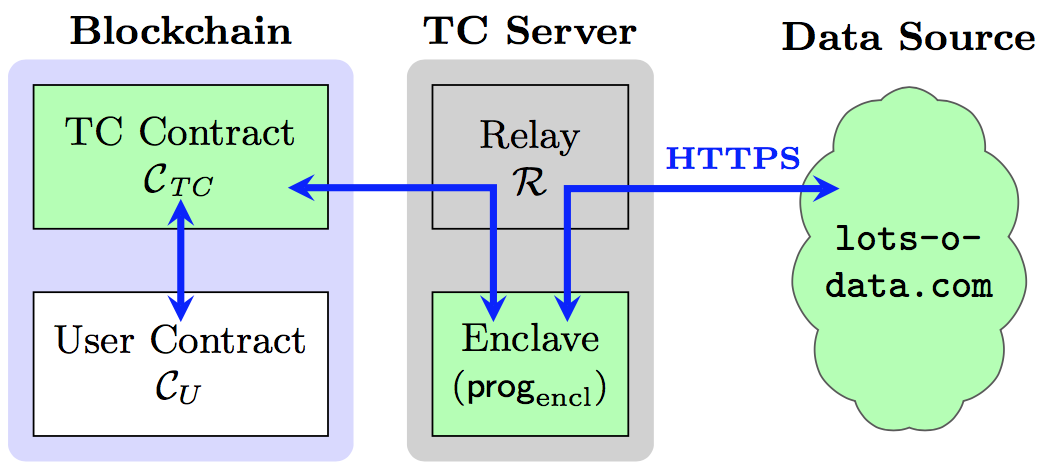
\includegraphics[width=0.7\textwidth]{figures/town-crier.png}
      \caption{Town crier Architecture.}
      \label{fig:/figures/town-crier2}
    \end{center}
\end{figure}



\subsubsection{Conclusions}
Town Crier, presents an effective solution to tackle trust issues in the oracle operation. It does require the use of proofs as well as its later analysis for good behaviour and specific hardware.

In scenarios, where there is a higher requirements for trust in the oracle behaviour and cost/performance is not a problem, TC is a viable and more secure solution than software-based proofs.


\section{Summary}

%FIXME: Falta aqui um texto a comparar as várias opções, se possível ilustrado por uma tabela de síntese em que se mostre rapidamente em que pontos são semelhantes e diferentes